\chapter{Uvod} \label{uvod}
Skozi celotno zgodovino so si ljudje želeli olajšati fizična dela na različne načine. Ponavljajoča dela je olajšala uporaba pogonov. Električni pogoni so delovne procese optimizirali.
Za točnejše delovanje so se razvili različni načini krmiljenja. Z novimi načini krmiljenja, so se pojavile potrebe po merjenju novih količin. V zadnjih desetletjih, je pri krmiljenuju pogonov, potrebna informacija
o trenutnem položaju pogona.

Trenutni položaj merijo dajalniki pomika ali zasuka\cite{uporabaSenzorjev}. Dajalnike zasuka se loči na dajalnike, ki merijo zasuk na koncu osi (angl.: on axis) in dajalnike, ki merijo zasuk na osi (angl.: through hole).
Možna delitev dajalnikov zasuka je tudi na eno-obratne (angl.: single-turn) in več-obratne (angl.: multi-turn). Eno-obratni dajalnikov zasuka podajo položaj znotraj enega obrata, medtem ko več-obratni
štejejo tudi število polnih obratov. Dajalnike položaja se deli glede na uporabljeni princip zaznavanja fizikalne
spremembe. Obstajajo magnetni, optični, induktivni in drugi \cite{killer}.

Pri magnetnem principu senzor dajalnika zaznava spremembo jakosti in smeri
gostote magnetnega pretoka ali polja. 
Gostoto magnetnega polja se povzroči z magnetnim akutuatorjem. Gostoto magnetnega polja se meri s Hallovimi sondami, AMR senzorji ipd.
Iz zajetega polja sledi izračun dejanskega položaja. Dajalnik položaja, ki pretvarja merjeno količino v informacijo se imenuje enkoder \cite{enkoder}.

Kot vsak merilni element, ima tudi magnetni enkoder napako. Napaka se lahko pojavi ob narobe merjenem magnetnem polju \cite{RLS3}. Napako lahko povzroči tudi napačno pomerjeno polje.
To se zgodi ob nepravilni montaži enkoderja ali magnetnega aktuatorja na os vrtenja. S poznavanjem vplivov nepravilne montaže na napako pomerjenega položaja, se napako lahko predvidi in odpravi.

Cilj naloge je analizirati kako različne napake pri montaži, vplivajo na napako v signalu kota.
Želi se predstaviti čimbolj preprost model, ki bo dovolj točno opisal dogajanje ob prisotnosti napake in to prekontrolirati.

\chapter{Senzor RM44}
Senzor RM44 je 13 bitni enkoder, primeren za merjenje zasuka rotirajočega pogona \cite{RM44}.
Enkoder se nahaja v robustem ohišju, zato je primeren za delovanje v težkem industrijskem okolju. % , pritrjenega na konec rotirajoče osi pogonskega sklopa.
Oblika izhodnega podatka, je prilagodljiva na sistem aplikacije v kateri bo uporabljen \cite{Ambrozic}. Izhod senzorja je lahko analogen v obliki sinusnega in kosinusnega signala ali linearno spreminjajče
se napetosti med potencialoma $GND$ in $VDD$ v odvisnosti od kota zasuka.
Izhod je lahko tudi v obliki inkrementalnih signalov A in B s katerih se lahko določi smer in relativni zasuk vrtenja ter signal Ri kateri določa referenčno točko. Izhod je možen tudi preko SSI vodila. Senzor ima
možnost nastavitev resolucije od 5 do 13 bitov na obrat \cite{AM8192} \cite{RM44}. Senzor na katerem so bile opravljene meritve je imel 12 bitno resolucijo in na voljo analogna signala sinus in kosinus. Točno ime senzorja je
RM44AC0001S20F2E10, v delu bo poimenovan okrajšano RM44.
\begin{figure}[ht]
	\centering
	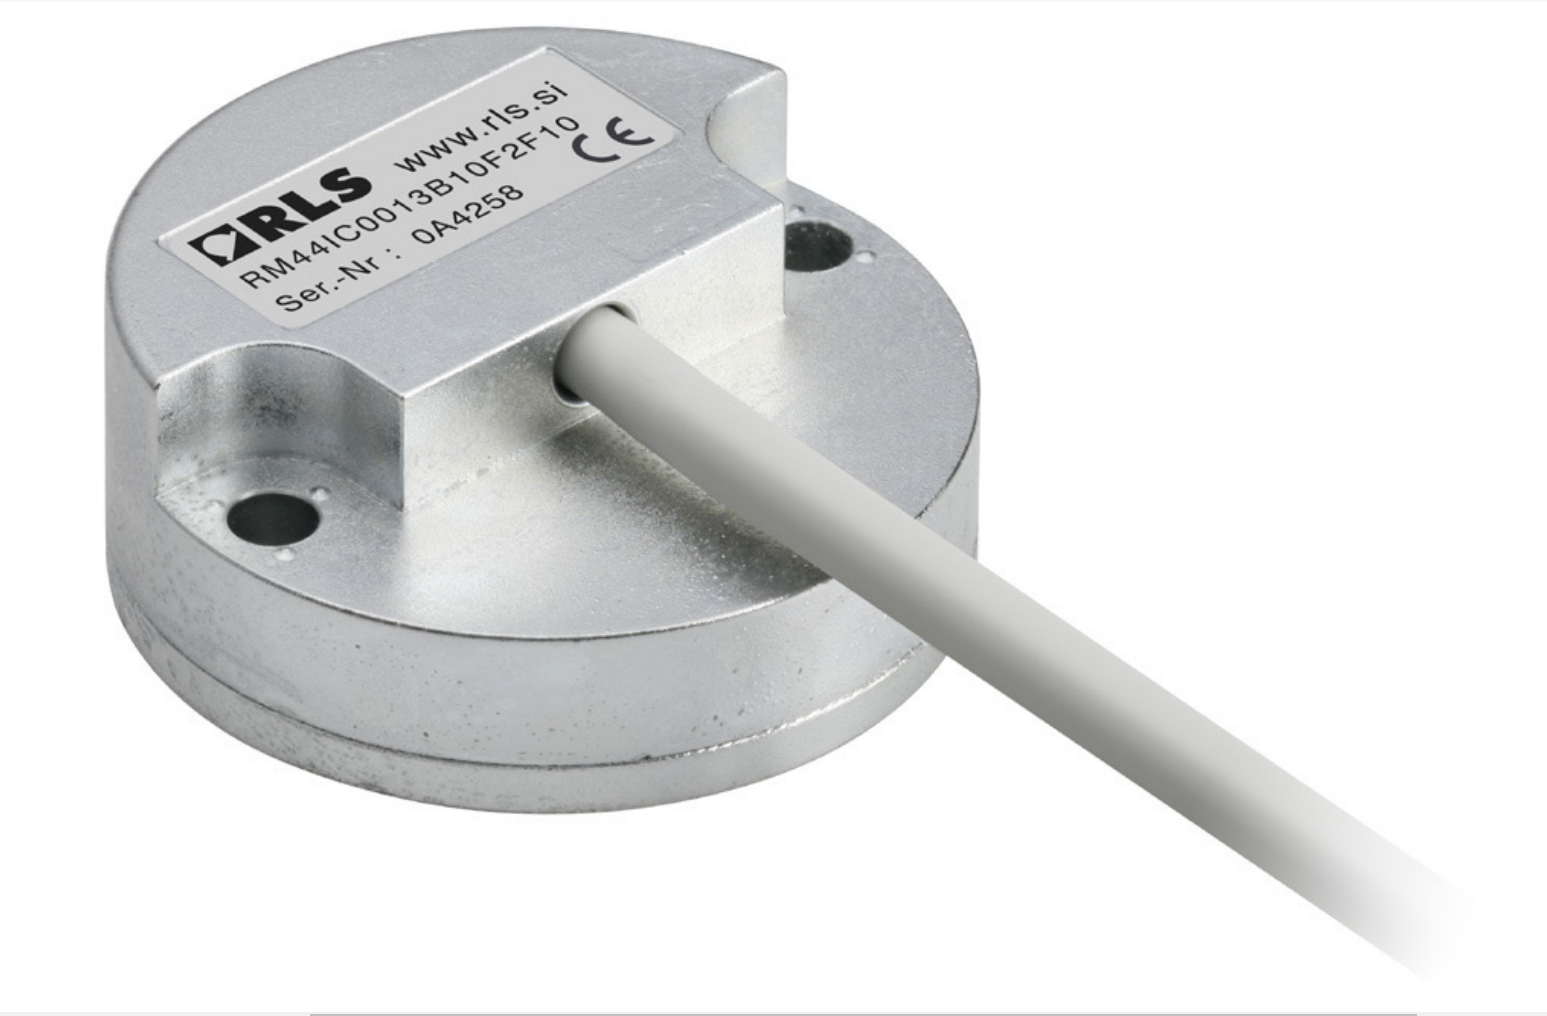
\includegraphics[width=0.6\columnwidth]{./Slike/senzorRM44.jpg}
	\caption{Senzor RM44}
	\label{RM44}
\end{figure}

Ključni element senzorja je čip AM256. Za pravilno delovanje, se mora nahajati nad radialno polariziranim cilindričnim magnetom, ki je pritrjen na os vrtenja (slika \ref{stranski_ris}).
S strani proizvajalca senzorja je priporočen radialno polariziran magnet s premerom 4 mm, višino 4 mm in remanenco 1050 mT (slika \ref{magnet4mm}).
\begin{figure}[ht]
	\centering
	\includegraphics[width=0.5\columnwidth]{./Slike/stranski_ris.png}
	\caption{Nahajanje radialno polariziranega magneta nad čipom AM256 \cite{AM8192}}
	\label{stranski_ris}
\end{figure}
\begin{figure}[ht]
	\centering
	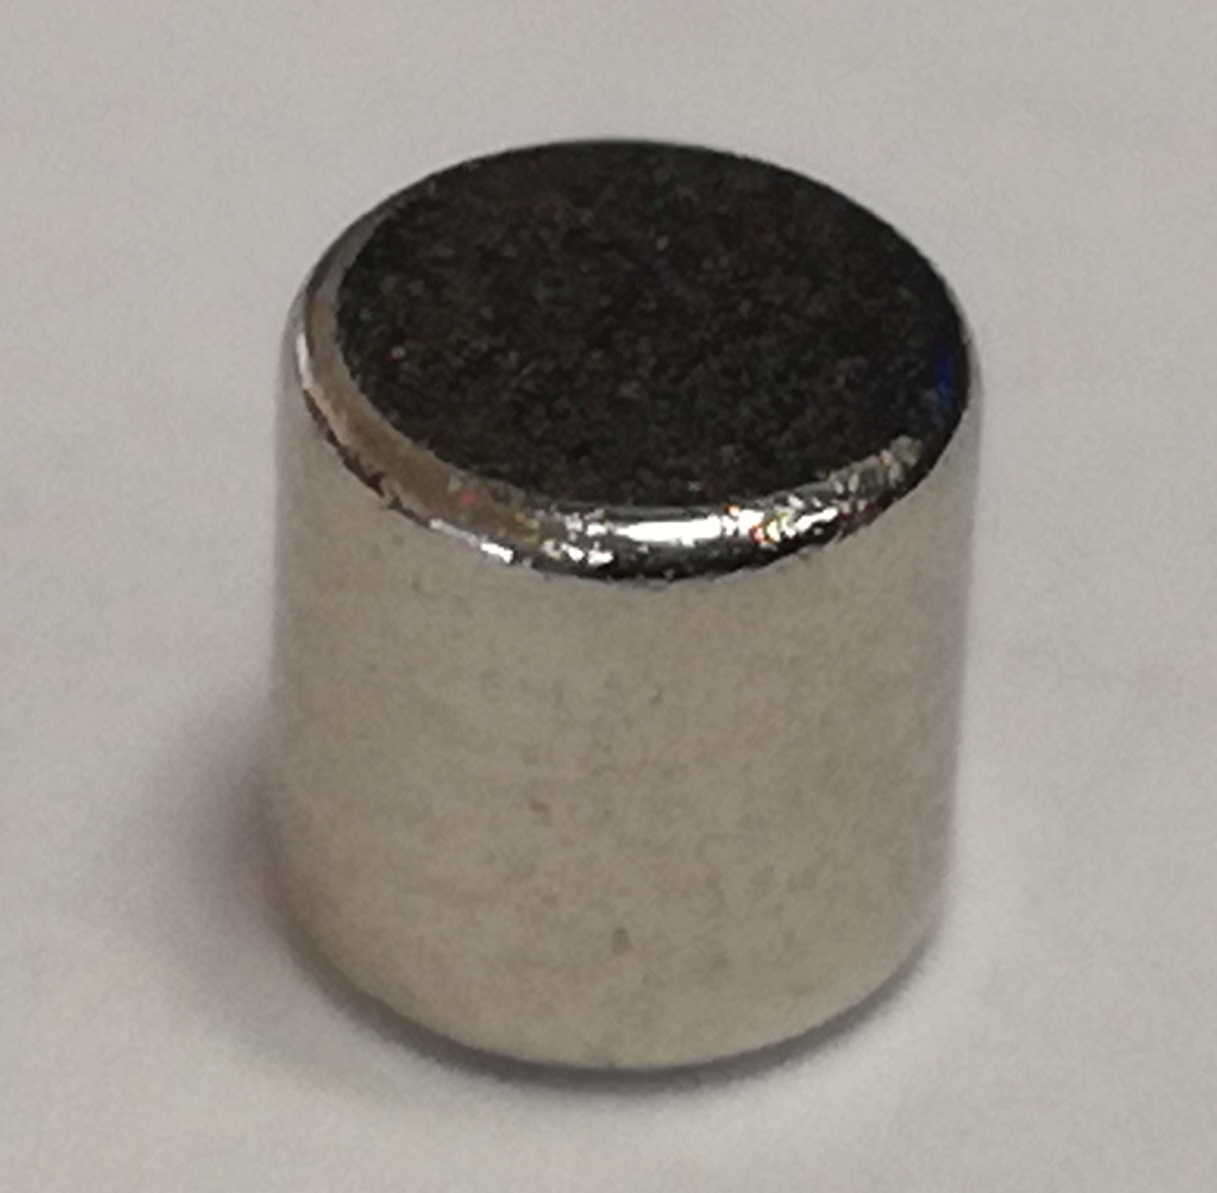
\includegraphics[width=0.35\columnwidth]{./Slike/magnet4mm.png}
	\caption{Primer magneta predlagan s strani proizvajalca RLS}
	\label{magnet4mm}
\end{figure}

Na siliciju čipa so razporejene Hallove sonde za meritev Z-komponento gostote magnetnega polja. Za merjenje Z-komponento gostote magnetnega polja je lahko čip obrnjen kot na sliki \ref{stranski_ris}, ali
obrnjen na glavo. Med silicijevo rezino in magnetom se pri taki montaži nahaja še tiskanina. Tiskanina nima magnetnih lastnosti in ne vpliva na Z-komponento gostote magnetnega polja povzročene z magnetnim aktuatorjem. Pri montiranju senzorja je potrebno ohraniti predpisano
razdaljo med magnetom in silicijevo rezino ($1,8 \mathrm{mm}$).

\begin{figure}[ht]
	\centering
	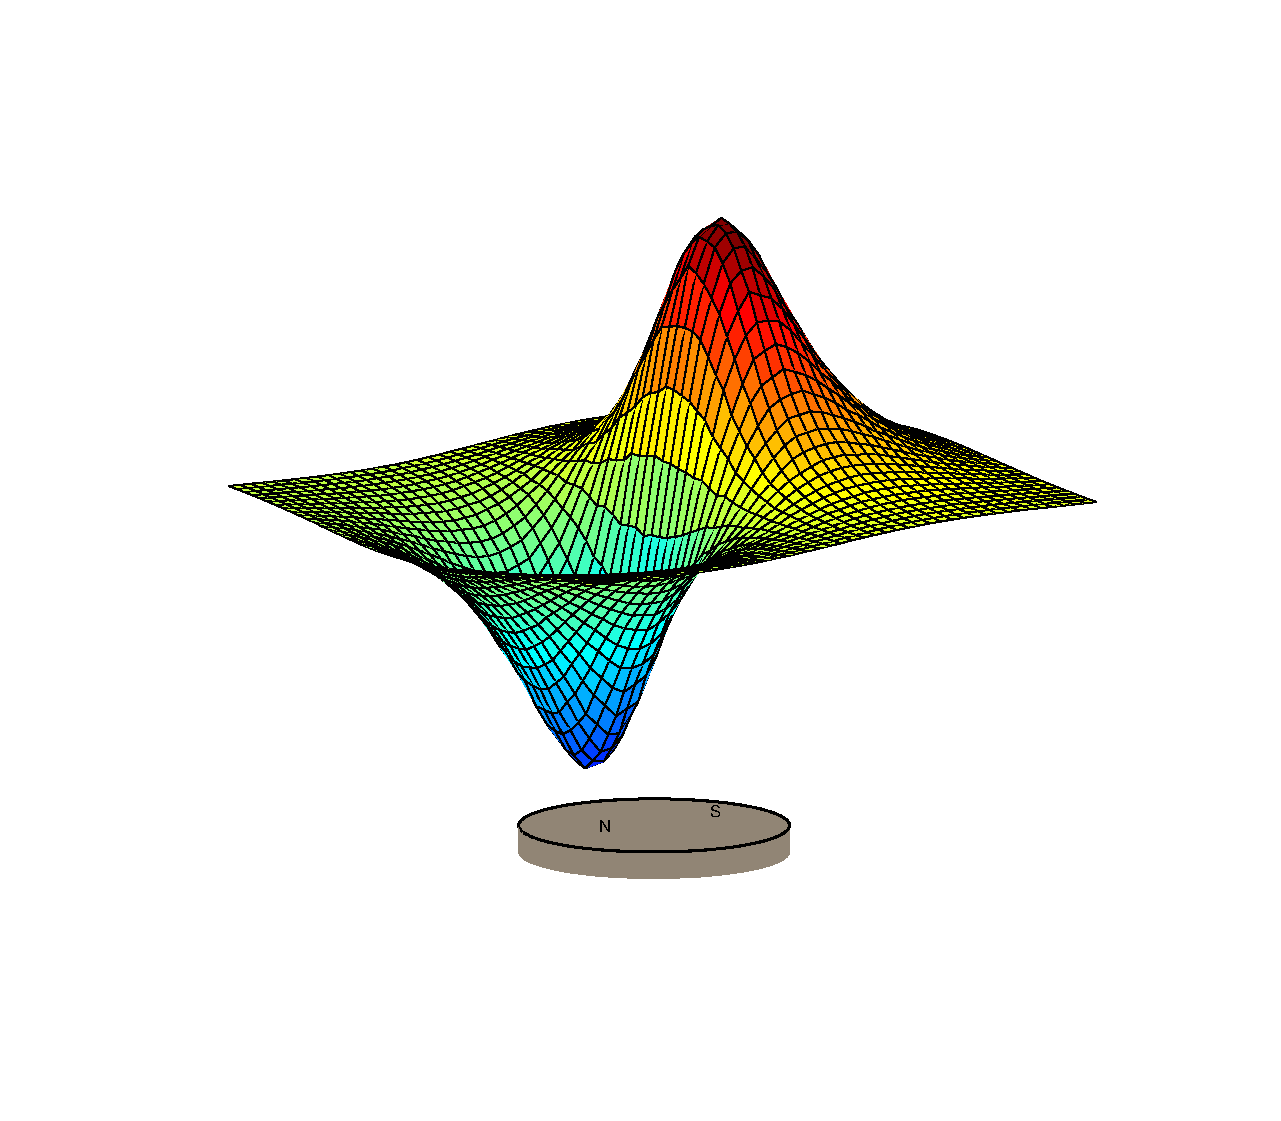
\includegraphics[width=0.9\columnwidth]{./Slike/polje_brez_ravnine.eps}
	\caption{Oblika Z komponente gostote magnetnega pretoka nad magnetom}
	\label{polje_brez_ravnine}
\end{figure}

Na sliki \ref{polje_brez_ravnine}  je prikazana oblika Z-komponente vektorja gostote magnetnega polja povzročene z radialno polariziranim cilindričnim magnetom.

S pravilno postavitvijo Hallovih sond in obliko Z-komponente gostote magnetnega polja povzročene z magnetom, se ob prostorskem zajemu zajame 2 signala kosinusne oblike, ki sta za 90$^\circ$ prostorsko zamaknjena
drug na drugega (slika \ref{BxBy}). Prvi zajet signal,  fazno prehiteva za 90$^\circ$ drugi signal in je v delu poimenovan $B_{cos}$, drugi signal, je poimenovan $B_{sin}$.
\begin{figure}[ht]
	\centering
	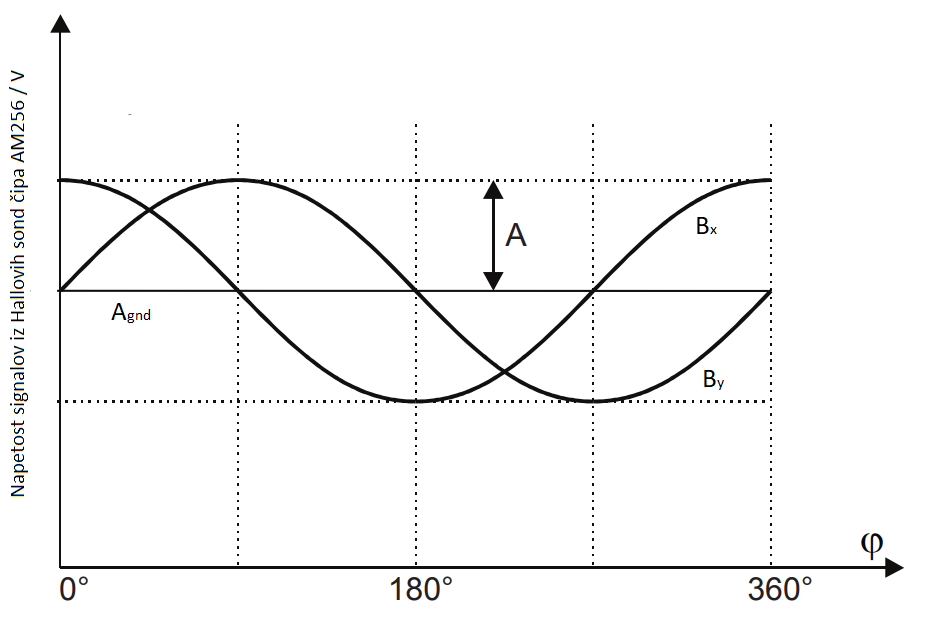
\includegraphics[width=0.75\columnwidth]{./Slike/BxBy.png}
	\caption{Analogna signala zajeta s Hallovimi sondami \cite{AM8192}}
	\label{BxBy}
\end{figure}

Iz signalov, zajetih s Hallovih sond, se izračuna kot. Metod, za numeričen izračun kota iz podatkov kot sta signala $B_{cos}$ in $B_{sin}$ je več (CORDIC, SAR, sledilna metoda, itd \cite{ICHaus_interpolate}). Osnovni
princip metode je izračun funkcije atan2($B_{sin}$, $B_{cos}$) \cite{atan2Matlab}.

Osnovno delovanje senzorja se lahko ponazori, s 4 Hallovimi. Sonde so enakomerno razporejene po krožnici s središčem v osi vrtenja in radijem  $r_0$. Z diferencialnim odčitavanjem pomerjenih signalov nasproti ležečih Hallovih sond, se signaloma $B_{sin}$ in $B_{cos}$ odstrani enosmerno komponento in poviša amplitudo.

Signala $B_{cos}$ in $B_{sin}$. sta vhodna parametra v funkcijo atan2(), ki izračuna kot zasuka (slika \ref{opis_modela}).
Za oceno napake, se lahko Z komponento gostote magnetnega pretoka v okolici središča magneta, aproksimira z ravnino (slika \ref{polje_z_ravnino}).

Aproksimacija zadostuje za oceno napake. S poznavanjem lokacije sonde glede na magnet, se lahko izračuna merjena komponenta magnetnega polja. Aprokisimirano polje je linearno odvisno od x komponente (\ref{equ:poljeB1}).
\begin{equation}
\label{equ:poljeB1}
B_z(x,y)=k\cdot x.
\end{equation} 
\begin{figure}[ht]
	\centering
	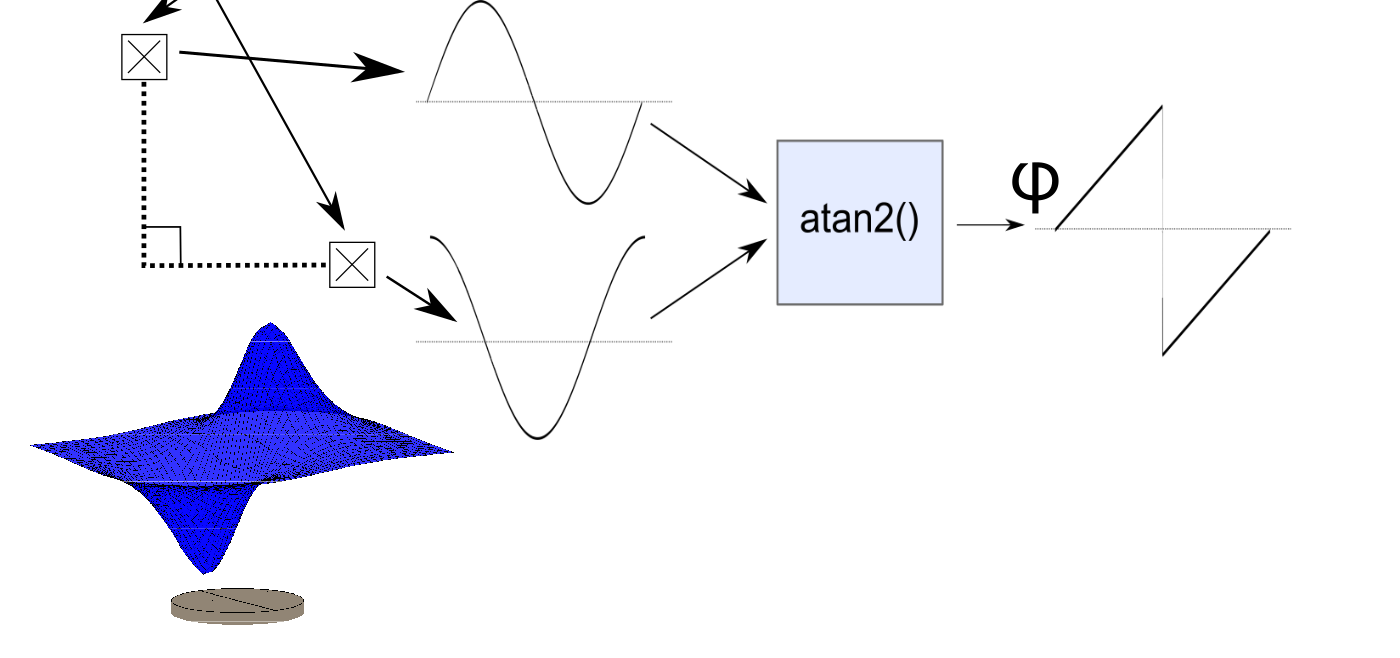
\includegraphics[width=0.9\columnwidth]{./Slike/opis_modela.png}
	\caption{Osnovni model, za izračun kot zasuka}
	\label{opis_modela}
\end{figure}
\begin{figure}[ht]
	\centering
	\includegraphics[width=\columnwidth]{./Slike/polje_z_ravnino.eps}
	\caption{Oblika Z komponente gostote magnetnega polja nad magnetom in aproksimirano ravnino v središču magneta}
	\label{polje_z_ravnino}
\end{figure}